% y = sin x と y = cos x のグラフ（0 ≦ x ≦ 2π）
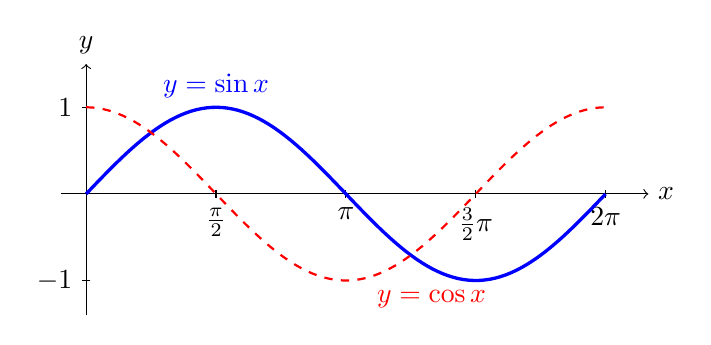
\begin{tikzpicture}[xscale=1.05,yscale=1.1]
  \draw[->] (-0.3,0) -- (6.8,0) node[right] {$x$};
  \draw[->] (0,-1.4) -- (0,1.5) node[above] {$y$};
  \foreach \x/\l in {1.5708/\frac{\pi}{2}, 3.1416/\pi, 4.7124/\frac{3}{2}\pi, 6.2832/2\pi}
    \draw (\x,0.05) -- (\x,-0.05) node[below] {$\l$};
  \draw (0.05,1) -- (-0.05,1) node[left] {$1$};
  \draw (0.05,-1) -- (-0.05,-1) node[left] {$-1$};
  \draw[very thick,blue,domain=0:6.2832,samples=100] plot (\x,{sin(\x r)});
  \draw[thick,red,dashed,domain=0:6.2832,samples=100] plot (\x,{cos(\x r)});
  \node[blue,above] at (1.5708,1) {$y=\sin x$};
  \node[red,below right] at (3.4,-1) {$y=\cos x$};
\end{tikzpicture}
